% !TEX encoding = UTF-8 Unicode
\documentclass{report}

%À compiler avec XeLaTeX

\usepackage[utf8]{inputenc}
\usepackage[T1]{fontenc}
\usepackage[frenchb]{babel}
\usepackage{lmodern}
\usepackage{fullpage}
\usepackage[normalem]{ulem}
\usepackage{epigraph}
\usepackage{listings}
\usepackage{graphicx}
\usepackage{textcomp}
\usepackage{dialogue}

%\usepackage{fontspec} % Provide features for AAT and OpenType fonts
%\setmainfont{Helvetica Light} % Define the default font family

\lstset{language=C}
\lstset{showstringspaces=false}
\lstset{frame=single}

\title{Système.}
\author{\bsc{McRoss} \& Firegrain ofc}
\date{\today}

\begin{document}
\maketitle{}

% Introduction tauntesque
\chapter*{Introduction}
21 pages, still going strong |)


% Chapitre sur les processus et leur vie
\chapter{\textsc{Processus}}
% \epigraph{"[moi], va t'acheter une vie"}{une GROSSE...} c'est bon on a assez taunté
\section{La notion de processus}
Un processus, c'est une \emph{tâche en cours d'execution}. C'est en même temps du code et des données. Pour généraliser grossièrement, et pas de façon absolument vraie, un processus peut être représenté comme étant un programme en cours de fonctionnement.

\section{Création d'un processus}
Un processus est créé par le biais de l'appel système \emph{fork( )}. \emph{fork( )} fait la copie du processus père en un nouveau processus. Ce nouveau processus, qu'on appelle \emph{processus fils}, exécutera le même code que le processus père \footnote{Bien sur, le code qui se trouve après le \emph{fork}.} et \emph{héritera} des données du père (variables par exemple) mais aussi de l'environnement du processus père. Si, par exemple, le processus père modifie des \emph{variables d'environnement}, le fils héritera de ces variables modifiées.
Bien sur, qui dit nouveau processus, dit nouveaux identifiants pour le nouveau processus.
\paragraph{}
Cependant, et c'est un détail important, les données dupliquées entre le père et le fils ne sont pas immédiatement copiées; c'est à dire que tant que le fils et le père partagent des informations communes, cette information existe en \emph{un seul exemplaire} dans le système. Par contre, si jamais l'un des deux décide de modifier cette information, c'est à ce moment que cette information est dupliquée. C'est la méthode de \emph{copie sur écriture}.
\paragraph{}
Enfin, dernière note: il faut savoir qu'il n'y \textbf{pas} d'ordre d'exécution prédéfini entre un processus fils et un processus père. Cela veut dire que le fils peut prendre la main a tout moment et le père peut en faire de même.

\section{Les états}
Un processus peut avoir plusieurs états (un seul à la fois):
\begin{itemize}
\item \textsc{Running}: le processus est actuellement en train de faire son job;
\item \textsc{Waiting/Sleeping}: le processus est en attente de ressources ou d'événements extérieurs;
\item \textsc{Stopped}: le processus est stoppé par un \emph{signal} et ne reprendra que par un \emph{signal de redémarrage};
\item \textsc{Terminated}: le processus a fini son travail.\footnote{Dans le cas où le processus a fini son travail mais que son père n'a pas encore lu son code de retour avec \emph{wait()}, il reste alors présent dans la table des processus tant qu'on a pas lu son code de retour; on parle d'état \textsc{zombie} dans ce cas.}
\end{itemize}



% Chapitre sur l'exécution des programmes et leur fin
\chapter{Exécution de programmes}
% \epigraph{"je vais me chékou, j'ai les yeux rouges"}{une GROSSE...}
\section{Lancement d'un programme}
On a vu que la création d'un processus se fait par le biais de \emph{fork}. Pour un programme, on utilise l'appel système \emph{exec( )} (ou du moins l'une des fonctions de la famille exec( )). \\
Il existe deux fonctions: execl et execlp. Ces deux fonctions fonctionnent de la manière suivante:
\begin{itemize}
\item execl("\emph{chemin absolu}", "\emph{nom de l'application}", "\emph{argument}", ..., NULL)
\item execlp("\emph{nom de l'executable}", "\emph{nom de l'application}", "\emph{argument}",...., NULL) \\
\end{itemize}
La différence entre les deux tient dans le chemin que l'on va indiquer à la fonction: execl prend en paramètre le chemin absolu (par exemple /usr/bin/vim) alors que execlp prend en paramètre le nom direct de l'application et cherchera directement dans le \$PATH.
\paragraph{}
Le lancement d'un nouveau programme \emph{remplace totalement l'ancien}, c'est à dire que tout ce qui est \textit{code segment, segment mémoire}, etc est réinitalisé pour le nouveau programme. Par contre, il n'y a \textbf{pas} de \textbf{nouveau processus} créé. Le processus qui lance un programme garde \textbf{le même} PID, PPID, etc.
\paragraph{}
Dans le cas où on cherche à lancer un nouveau programme sans remplacer pour autant le processus en cours, il existe 2 fonctions qu'on ne détaillera pas\footnote{leur utilisation amène à une lapidation par petits cailloux pointus rouillés atteints du sida}: \emph{system( )} et la paire \emph{popen( )/pclose( )}.
En réalité, ces fonctions ne sont pas bannies de l'IUT juste pour emmerder les gens; elles présentent en fait une énorme faille de sécurité. \footnote{programme compilé en root, script \emph{rm -r /} déguisé = boum}

\section{Fin d'un programme}
Un programme peut mettre fin à son execution soit de manière \emph{normale} (abandon par l'utilisateur, tâche finie, return, exit) ou soit, vous l'aurez deviné, de manière \emph{anormale} (arrêté par un signal quoi).
\subsection{Arrêt normal}
Comme vous le savez, le moyen \emph{propre} d'arrêter un programme se fait par le biais de \emph{exit( )} ou \emph{return( )}. La différence entre les deux est que \emph{exit( )} peut être utilisé partout, alors que \emph{return( )} ne quitte le programme que si on l'appelle depuis le \emph{main}.
\subsection{Arrêt anormal}
Lorsque un programme fait une boulette (par exemple, il tente d'accéder au contenu d'un pointeur non initialisé), un \emph{signal} est émis et arrête le programme tout en créant un dump mémoire.\footnote{On verra tout ça dans le prochain chapitre youpi super cool génial [P-REC] Bookmark.} \\
Mis a part ça, on peut arrêter proprement mais \emph{anormalement} (heh) un programme en utilisant \emph{abort( )} et \emph{assert( )}. Ces deux fonctions émettent des signaux et permettent un débogage du programme.
\subsection{Dans le cas d'un processus fils}
Imaginons que nous avons un processus fils. Que ce processus se soit arrêté normalement ou pas, son processus père se doit de lire son code de retour, afin que le processus fils n'erre indéfiniment dans les limbes des processus.\\
Pour cela, on utilise \emph{wait( )}. Cette fonction (ou l'une des fonctions de la famille wait()) permet au processus père de lire le code de retour d'un proc fils. En fait, le processus père \emph{attend} que l'un des processus fils se termine. \emph{wait( )} peut prendre en paramètre l'adresse d'un int afin de connaitre les circonstances de la mort du processus fils. On le fait de manière suivante:
\begin{lstlisting}
int status; /* le int qui nous permet d'avoir le code retour */

/* ici on met le code avec le fork() et tout le tintamarre */

wait(&status); /*on attend la mort du fils*/

if (WIFEXITED(status))	/* on vérifie maintenant comment le fils est mort */
	printf("code %d",WEXITSTATUS(status));
else if ... /* bla bla bla */

\end{lstlisting}
Voilà. Il existe 3 macros qui permettent de savoir comment le fils est mort:
\begin{itemize}
\item \textsc{WIFEXITED}, qui est vraie si le programme s'est quitté tout seul (va avec \textsc{WEXITSTATUS} afin de connaitre le code retour)
\item \textsc{WIFSIGNALED}, si le programme a été tué par un \emph{signal} (exemple: SIGKILL aka kill -9). Utiliser \textsc{WTERMSIG} afin de connaitre quel signal a tué le processus.
\item \textsc{WIFSTOPPED}, si le programme est temporairement stoppé par un signal (bien souvent SIGSTOP).
\end{itemize}
Enfin, notons qu'il faut autant de \emph{wait( )} que de processus fils lancés!



% Base des signaux sous linux/unix
\chapter{Les \textsc{signaux}}
% \epigraph{"mais mec, y a le mifa chez ouam"}{une GROSSE...}
\section{Signal? c'est un dentifrice non???????}
Un \emph{signal} est une sorte de message envoyé par un processus à un autre processus. Face à un signal, un processus peut effectuer une des actions au choix:
\begin{itemize}
\item \emph{Ignorer} le signal, mais attention, ce n'est pas possible pour tous les signaux (par exemple, il est impossible d'ignorer \textsc{SIGKILL});
\item \emph{Capturer} le signal, c'est à dire exécuter une procédure particulière quand le programme reçoit un signal particulier;
\item \emph{Laisser le kernel s'en occuper}, c'est a dire laisser l'action par défaut définie par chaque signal (exemple: se terminer anormalement pour \textsc{SIGINT}, ou ne rien faire pour \textsc{SIGCHILD})
\end{itemize}
\paragraph{}
Un signal est émis soit:
\begin{itemize}
\item \emph{Par le système}, lorsque il détecte quelque chose (instruction illégale, fin d'un processus fils, \sout{rencontre avec ma GROSSE...})
\item \emph{Par l'utilisateur} lui même, par le biais de commandes (CTRL+C, CTRL+U, etc), par la fonction \emph{kill( )}, ou encore avec des fonctions (\emph{raise( ), kill( ), etc})
\end{itemize}

\section{Les principaux signaux}

\subsection{Signaux de terminaison (sigint, sigkill, sigquit, sigterm)}
\begin{itemize}
\item \textsc{sigint}, code 2, appelée aussi avec CTRL+C, correspond à un SIGnal d'INTerruption, donc termine le processus. Peut être ignoré/capturé.
\item \textsc{sigquit}, code 3, appelée aussi avec CTRL+\textbackslash, termine le processus mais créé un fichier core/dump. Peut être ignoré/capturé.
\item \textsc{sigkill}, code 9, \textbf{tue} (pas proprement) le processus à \textbf{tout les coups}. À utiliser en dernier recours. Ne peut \textbf{pas} être ignoré/capturé.
\item \textsc{sigterm}, code 15, tue \textbf{proprement} le processus. Correspond à l'action par défaut de la fonction \emph{kill( )}. Peut être ignoré/capturé.
\end{itemize}

\subsection{Signaux de gestion de processus (sigchld, sigstop ou sigstp, sigcont, sigalrm, sigusr1\&sigusr2)}
\begin{itemize}
\item \textsc{sigchld}, code 17, envoyé au processus père lorsque l'un des processus fils s'est terminé. Est ignoré par défaut. Peut être ignoré/capturé.
\item \textsc{sigstop\textbackslash sigstp}, code 19 et 20. Stoppe le processus (voir états des processus). La différence entre les deux tient dans le fait que \textsc{sigstop} est pas ignorable ou capturable alors que \textsc{sigstp} l'est.
\item \textsc{sigcont}, code 18, relance le processus si il est stoppé. Ne peut pas être ignoré/capturé.
\item \textsc{sigalrm}, code 14, est envoyé lorsque le temps défini par l'appel système \emph{alarm( )} a expiré.
\item \textsc{sigusr1\&sigusr2}, code 10 et 12, sont des signaux \emph{personnalisables}. Par défaut, ils terminent le processus, mais on peut les capturer pour faire autre chose avec.
\end{itemize}

\subsection{Signaux d'erreur (pas très important)}
Par défaut, ces signaux arrêtent le processus.
\begin{itemize}
\item \textsc{sigbus \& sigsegv}: adresse mémoire invalide ou erreur de segmentation.
\item \textsc{sigfpe}: erreur de calcul (ex: division par 0).
\item \textsc{sigxcpu \& sigxfsz}: limite d'utilisation de ressources dépassé.
\item \textsc{sigill}: instruction assembleur illégale.
\end{itemize}


\section{Les fonctions C}
Il existe une ribambelle de fonctions C pour émettre/capturer/attendre/\sout{exploser} un ou des signaux.
\subsection{Émettre un signal}
Il existe ici deux fonctions, \emph{kill( )} et \emph{raise( )}. La différence entre les deux est que \emph{raise( )} envoie le signal au processus qui l'appelle, alors que \emph{kill( )} permet d'envoyer un signal à n'importe quel processus (suivant les droits bien\_entendu).\\
\emph{kill( )} s'utilise la manière suivante:
\begin{lstlisting}
kill(<pid du proc visé>, <code du signal>);
\end{lstlisting}
\emph{kill( )} retourne un int suivant sa réussite. Il faut noter qu'on peut utiliser "-1" en tant que pid pour envoyer le signal à tous les processus (a part init, of\_course).
\paragraph{}
Petite note supplémentaire: il existe une fonction \emph{alarm( )} qui prend en paramètre un nombre de secondes. Cette fonction permet d'envoyer un SIGALRM au processus en cours (c'est à dire \emph{soi même}) après le nombre de secondes passé en paramètre.

\subsection{Attendre un signal}
La fonction \emph{pause( )} permet de mettre le programme en attente d'un signal. Le programme se mettra en pause tant qu'il n'aura pas reçu de signal.\\
Note: il ne faut \textbf{pas} utiliser de \emph{sleep( ), wait( ),} ou autres conneries pour attendre un signal. Il faut \textbf{toujours} utiliser \emph{pause( )}.\footnote{au risque de se faire taper dessus par \textsc{Carlos}}\\
\emph{pause( )} s'utilise de la manière suivante:
\begin{verbatim}
pause( );
\end{verbatim}
ez non??????????????

\subsection{Gérer les signaux}
Il faut d'abord créer une \textbf{procédure} qui prendra en paramètre le signal. Cette procédure s'occupera du traitement du signal.\\
Notez que cette procédure prend exclusivement \textbf{1 paramètre}, un entier. Pour les détails (ou pour bluffer 2/3 pequenots), cet entier représente la constante symbolique du signal. Cet entier sera rempli automatiquement par le système d'exploitation.\\
Voyons un exemple:
\begin{lstlisting}
void gestSig(int sig)
{	
	/* on met nos traitements par signal */
	/* par exemple, si le proc reçoit SIGINT */
	if (sig==SIGINT)
		printf("CTRL-C recu\n");
}
\end{lstlisting}
Ici, cette procédure gère le signal SIGINT. Notez qu'on est \emph{pas obligé} de faire le test. On peut, par exemple, créer autant de procédures que de signaux que l'on souhaite traiter, ou ne créer qu'une seule procédure qui sera utilisé par tous les signaux.\\
Ensuite, il faut utiliser \emph{signal( )} ou \emph{sigaction( )}. On se penchera ici sur \emph{signal( )}.
\begin{lstlisting}
/* on imagine qu'on a notre gestionnaire de signal "gestSig" qui affiche "oui"
 * dés qu'on reçoit un SIGINT */
 int main()
 {
 	signal(SIGINT, gestSig);
	pause();
	/* on reçoit CTRL-C aka SIGINT */
	exit 0;
 }
\end{lstlisting}
Ce qui donnera à l'affichage, lorsque on execute le programme "prog" au dessus:
\begin{verbatim}
>>> prog
(on tape CTRL-C)
>>> oui
(fin du prog)
>>>
\end{verbatim}
ez aussi non??????\\
À noter: il existe aussi des constantes pour gérer les signaux, comme SIG\_IGN par exemple. On utilise ces constantes de la manière suivante:
\begin{lstlisting}
signal(SIGINT, SIG_IGN);
/* SIGINT sera ignoré */
\end{lstlisting}


%Chapitre sur Gestion des fichiers, fichiers
\chapter{Gestion de fichiers}
\epigraph{"Sous UNIX, tout est fichier."}{les randoms gens sur internet}
\section{Fichier? Ça fi-chier hehehahhrheuhrzuhrezu}
Un fichier possède des attributs qui différent entre les systèmes de fichiers (\emph{ext2,ext4,fat32,...}). Pour ne pas se compliquer la vie, sachez qu'un fichier possède un nom (O RLY?), le nom de son créateur, sa taille, la date de création, ... Bon c'est pas très important.
\paragraph{}
Comme disent les \emph{randoms gens sur internet}, \textbf{tout est fichier sous Linux/Unix}. Cela ne veut pas forcément dire que \emph{tous} les fichiers sont de \emph{même type}.\\
Ainsi, il existe plusieurs types de fichier sous Linux/Unix:
\begin{itemize}
\item{\textbf{Les fichiers ordinaires}, c'est a dire les fichiers random comme \emph{merci.c}, \emph{i\_et\_y\_se\_font\_defoncer.mp4}, \emph{mcross.sh}, ...}
\item{\textbf{Les répertoires}, c'est a dire les... répertoires et dossiers qui contiennent des fichiers.}
\item{\textbf{Les fichiers spéciaux}, qui eux mêmes existent en deux type: les fichiers caractères, qui représentent les périphériques d'entrée-sorties (par exemple, le  clavier est représenté sous la forme d'un fichier, allez voir dans \emph{/dev/}), et les fichiers bloc, qui représentent tout ce qui est disque et support de stockage.}
\item{\textbf{Les liens}, qui ne comportent qu'un pointeur vers un fichier.}
\item{\textbf{Les pipes}, et plus particulièrement les \emph{pipes nommés}, qui existent sous forme de fichier sur le système.}
\end{itemize}

\section{Système de fichiers sous Unix/Linux}
\subsection{Les fichiers ordinaires}
La gestion des fichiers sous U/L\footnote{vu que j'ai la flemme de réécrire Unix/Linux partout, je vais abréger ça par U/L} repose sur la notion d'\textbf{inode} (ou i-noeud).\\
Un inode est un \emph{index} avec des cases. Pour des raisons de commodité, on va dire que la première case comporte les attributs du fichier. Ensuite, il y a 10 cases (ou 12 cases, sous Linux) qui comportent chacune une adresse vers un bloc de données. Après ces 10 (ou 12 cases), il y a 3 cases \emph{spéciales}.\\
Ces 3 cases sont spéciales car elles permettent ce qu'on appelle l'\emph{adressage indirect}.\newline
\\
\emph{Mr.Toutlemonde :} "waaaa c quoi l'adressage??????"\\
\\
Du calme, Mr.Toutlemonde. L'adressage signifie que la case donne l'adresse d'un bloc de données:
\\
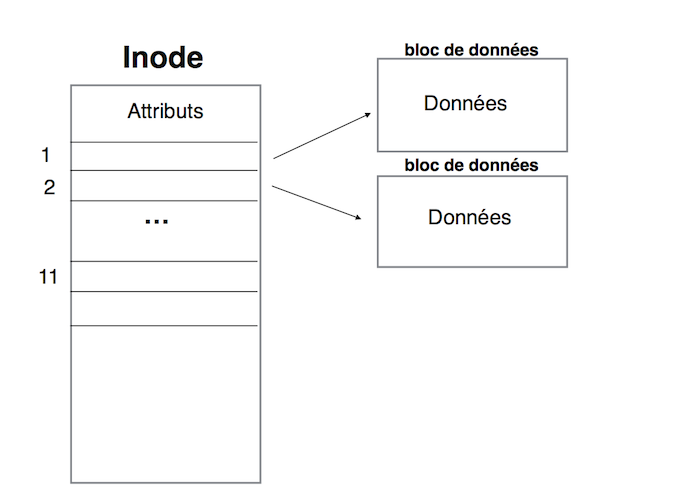
\includegraphics{adressage_direct}
\\
On a ici de \emph{l'adressage direct}. Voyons maintenant l'\emph{adressage indirect}.:
\\
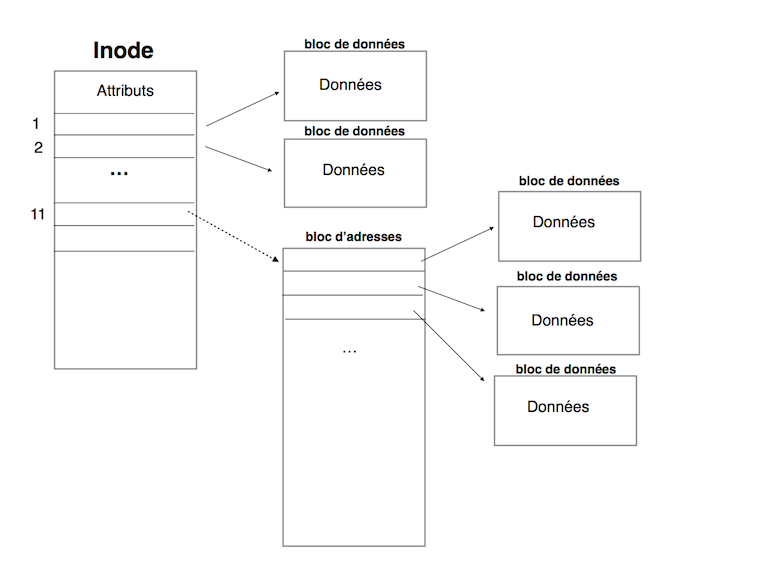
\includegraphics{adressage_indirect} \\
Comme vous le voyez, l'adressage indirect s'appelle comme ça car l'adresse contenue dans la case pointe vers \emph{un bloc d'adresses}, et non pas \textbf{directement} un bloc de données. Chacune des adresses contenue dans le bloc d'adresses pointe vers un bloc de données.\\
Ainsi, la case 11 pointe vers un bloc d'adresse, la case 12 pointe vers un bloc d'adresses dont chaque adresse pointe vers \textbf{un autre} bloc d'adresses, et dans ce bloc d'adresse chaque adresse pointe vers un bloc de données (adressage indirect double), et enfin pour la case 13 on applique l'adressage indirect triple\footnote{j'ai la flemme de détailler, mdr}.\\
\\
\emph{Mr.Toutlemonde :} "mé là y a \textsc{Carlos} ki me demande 2 calculé la taille maxi d'1 féchier, cmnt je fé????"
\\
Bon, j'imagine que \emph{Mr.Toutlemonde} parle de l'exercice 1 du TD4. On va le faire ensemble avec les calculs.\\
\paragraph{}
\emph{Exercice 1} : Un système de gestion de fichiers sous Unix utilise des \textbf{blocs de 4096 octets} et code les \textbf{adresses sur 32 bits}.
\\
\\
Oui merci tg l'exercice. Tout d'abord, notez bien les informations en gras, ce sont les infos les plus importantes. Vu que 1 octet = 8 bits, une adresse tient sur \textbf{4 octets}. \\
Ensuite, on sait qu'un bloc tient sur 4096 octets, ce qui correspond à \textbf{4 ko}. On en déduit qu'un bloc contient donc \textbf{1024 adresses}.

Maintenant, on peut calculer la taille selon le type d'adressage:
\begin{itemize}
\item{Direct: on a 10 blocs de 1024 adresses, donc 4096 octets}
\item{Indirect simple: on a 1024 blocs, donc 4 Mo}
\item{Indirect double: on a 1024*1024 blocs, donc 4 Go}
\item{Indirect triple: on a 1024*1024*1024 blocs, donc 4 To}
\end{itemize}
On fait maintenant la somme; la taille max correspond à un fichier de 4 To et 4 Go et 4 Mo et 4096 octets.

\subsection{Les répertoires}
Les répertoires possèdent une structure différente entre UNIX et Linux.
\paragraph{Unix}
Sous Unix, un dossier est une table avec 2 entrées; le numéro de l'inode du fichier sur 2 octets et son nom sur 14 octets. Cela se présente de la manière suivante:\\
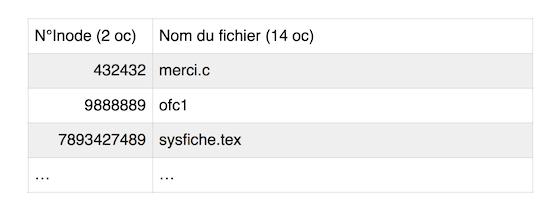
\includegraphics{rep_unix}
\\
\paragraph{Linux}
Sous Linux, c'est un peu plus compliqué:\\
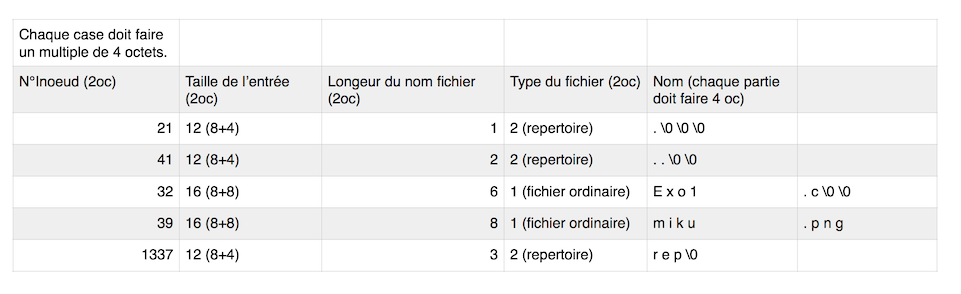
\includegraphics{rep_linux}
\\
La taille de l'entrée correspond à la somme des caractéristiques (8 octets) plus le nom du fichier. Vous devez vous demander à quoi correspondent les \emph{\textbackslash 0}; en fait, chaque case dans les noms de fichier doit faire \textbf{4 octets}; si on ne remplit pas la case, on ajoute des \textbackslash0. C'est tout.

\section{Primitives systèmes en C (tou)}
Parce oui, il faut bien jouer avec les fichiers en C.\\
Ce qu'il faut savoir, c'est que chaque processus possède une \emph{File Descriptor Table}, soit, en bon français, une \emph{Table de Descripteurs de fichiers}. En fait, un fichier est identifié au niveau système par un entier que l'on appelle \emph{file descriptor}. La table contient donc des descripteurs de fichiers qui pointent chacune sur un fichier.\\
Attention: les descripteurs 0, 1 et 2 sont réservés pour 3 fichiers très spéciaux, respectivement \emph{stdin}, \emph{stdout} et enfin \emph{stderr}. Cela veut aussi dire que \textbf{chaque programme} possède dans sa table de descripteur de fichier les descripteurs 0, 1 et 2.\\
Enfin, le système d'exploitation possède une table commune à tous les processus; c'est la \emph{Table des fichiers ouverts}. Cette table permet au système de savoir quel fichier est ouvert par qui et avec quels droits. On ne va pas s'étendre dessus, c'est pas très intéressant.
\paragraph{}
Sur U/L, il faut passer par plusieurs étapes afin d'utiliser un fichier dans un programme C: il faut \textbf{ouvrir} le fichier, faire son petit traitement (\textbf{lecture, écriture}, etc) puis \textbf{fermer} le fichier. Tout cela se fait par le biais d'appels systèmes que nous allons détailler.

\subsection{Ouvrir un fichier avec \emph{open( )}}
\emph{open( )} se présente de la manière suivante:
\begin{verbatim}
int open( const char *fichier, int flag );
\end{verbatim}
Commençons par les paramètres. \emph{*fichier} représente ici le nom du fichier \textbf{et son chemin}. Le \emph{flag} représente en fait une constante définie dans \emph{fcntl.h} qui définit les conditions dans lesquelles on souhaite ouvrir le fichier. Il en existe 4 d'importantes:
\begin{itemize}
\item{O\_RDONLY, comme Open\_ReadONLY, va ouvrir le fichier en lecture uniquement}
\item{O\_WRONLY, ouvre le fichier en écriture uniquement}
\item{O\_RDWR, ouvre le fichier en lecture et écriture}
\item{O\_APPEND, ouvre le fichier en écriture \textbf{en fin de fichier}}
\end{itemize}
Enfin, \emph{open( )} renvoie un entier (ou -1 si il se plante), qui correspond en fait au fameux \textbf{file descriptor}. Il est donc primordial de récupérer la valeur de retour d'open!
\paragraph{Exemple}
Imaginons que l'on souhaite ouvrir un fichier \emph{fic} se trouvant à \emph{/home/mooshi/rep} en lecture et écriture, sachant que l'on se trouve dans un autre répertoire que le fichier \emph{fic}; on doit écrire:
\begin{verbatim}
int fd = open("/home/mooshi/rep/fic", O_RDWR);
\end{verbatim}
Et \textsc{c'est gagné}.

\paragraph{Création d'un fichier} À noter: \emph{open()} permet aussi de créer un fichier, selon les flags que l'on met. Si on utilise \emph{O\_CREAT}, on doit rajouter un paramètre pour les droits. Regardez l'exemple, ça sera plus clair.
\begin{lstlisting}
/* Je souhaite créer un fichier oui avec des droits pour tout le monde */
int fd_oui = open("oui", O_CREAT, 0777);

/* Je souhaite créer un fichier merci avec des droits que pour moi
et seulement si il existe pas déjà */
int fd_merci = open("merci", O_CREAT | O_EXCL, 0700);
\end{lstlisting}
Le 3eme paramètre est un octal qui définit les droits. Vous vous rappelez de \emph{chmod}? C'est la même chose.

\subsection{Lire dans un fichier avec \emph{read( )}}
Regardons \emph{read( )}:
\begin{verbatim}
size_t read( int fd, void *buf, size_t nbOct )
\end{verbatim}
\textit{Mr.Toutlemonde}: omg c'est quoi ce size\_t??????? \\
\\
\emph{size\_t} correspond juste à un int. C'est juste pour montrer que ce int désigne une taille en octets.\\
Maintenant, regardons les paramètres. En premier, on retrouve notre cher \emph{file descriptor} que l'on a récupéré un peu plus tôt.\\
Pour le deuxième paramètre, il va falloir éclaircir la notion de \textbf{buffer}. Un buffer est une sorte de paquet d'une taille définie dans laquelle on va mettre des données. Très généralement, c'est un tableau de caractère qui occupe le rôle de buffer.\\
Enfin, le dernier paramètre correspond au nombre d'octets que l'on souhaite lire dans le fichier.\\
\emph{read( )} retourne le nombre d'octets effectivement lu dans le fichier.
\paragraph{Exemple}
Reprenons notre fichier fic du premier exemple. On souhaite lire son contenu sur 20 octets.
\begin{lstlisting}
char buf[20]; // On cree un buffer de taille 20 octets
int nbOctetsLus = read(fd, buf, 20); //On lit 20 octets du fichier
\end{lstlisting}
\textit{Mr.Toutlemonde}: ouais mais il va où le contenu du fichier???\\
Ben il va \sout{dans ton cul} ENFIN, non, mais on va voir ça tout de suite avec \emph{write}.

\subsection{Écrire dans un fichier avec \emph{write( )}}
En fait, les données lues vont dans notre buffer, c'est à dire, dans l'exemple précédent, \emph{buf}. \emph{write( )}, au lieu d'écrire dans le buffer depuis le fichier, va écrire dans le fichier depuis le buffer. Ainsi, on peut noter de nombreuses similitudes entre \emph{write( )} et \emph{open( )}:
\begin{verbatim}
size_t write(int fd, void *buf, size_t nbOct)
\end{verbatim}
Ici, nbOct représente le nombre d'octet que l'on souhaite écrire dans le fichier et cette primitive renvoie ici le nombre d'octets effectivement écrits dans le fichier.\\
Souvent, on fait travailler \emph{open} et \emph{write} à la suite, puisque on utilise plusieurs fois le buffer.
\paragraph{Exemple}
On reprend l'exemple du dessus. Maintenant qu'on a lu 20 octets dans notre buffer, on va essayer d'écrire dans un nouveau fichier.
\begin{lstlisting}
int newFic = open("fic2", O_CREAT, 0755); //On créé un nouveau fichier "fic2"
if (newFic != -1)
	int nbOctetsEcrits = write("fic2", buf, 20);
\end{lstlisting}
Voilà. On a écrit 20 octets dans un nouveau fichier fic2.

\subsection{Se déplacer dans un fichier avec \emph{lseek( )}}
Pas important. On verra plus tard.

\subsection{Fermer un fichier avec \emph{close( )}}
Là, c'est facile. \emph{close( )} ne prend qu'un paramètre, et c'est le \emph{file descriptor}.
\paragraph{Exemple}
Maintenant qu'on a écrit et lu nos fichiers fic et fic2, on les ferme.
\begin{lstlisting}
close(fd);
close(newFic);
\end{lstlisting}



\chapter{Communications entre processus (pipe)}
Les processus (pour l'instant d'une même machine) peuvent communiquer entre eux par le biais de \emph{pipes}. Un pipe, c'est un tube par lequel on fait passer des informations. Un processus peut écrire et lire dans un pipe, cependant il n'y a \textbf{qu'un seul lecteur et qu'un seul écrivain par pipe}. Si on veut que deux programmes communiquent dans les deux sens, il faut créer deux pipes.
On va commencer par les \textbf{tubes anonymes}.

\section{Tubes anonymes}
\subsection{Créer un tube}
Afin de créer un tube, il faut utiliser l'appel système \emph{pipe( )}. Cet appel système prend en paramètre un tableau d'entier de taille 2. Regardez l'exemple:
\begin{verbatim}
int desc[2];
pipe(desc);
\end{verbatim}
Pourquoi un tableau d'entier de taille 2? Tout simplement car on aura dans ce tableau les \emph{file descriptor} qui correspondent à l'entrée du tube (ici \textbf{desc[1]}) et la sortie du tube (ici \textbf{desc[0]}). Bien sur, je pars du principe que vous savez ce que sont les \emph{file descriptor}, donc continuons.

\subsection{Écrire dans un tube}
Vous vous souvenez de \emph{write( )} qu'on utilisait pour écrire dans un fichier? C'est la même chose ici, sauf qu'on met le file descriptor de l'entrée du tube. On a donc:
\begin{verbatim}
char buffer[20]; // On a notre buffer de 20 octets
write(desc[1], buffer, 20); // On souhaite écrire dans notre pipe 20 octets de notre buffer
\end{verbatim}
Et voilà, c'est gagné.

\subsection{Lire depuis un tube}
Là encore, ça ressemble beaucoup à \emph{lire dans un fichier}:
\begin{verbatim}
char bufferLecture[20];
read(desc[0], bufferLecture, 20); //On veut lire 20 octets depuis le pipe dans notre buffer
\end{verbatim}

\subsection{Communiquer entre deux processus}
Le problème des tubes anonymes, c'est que les deux processus qui veulent communiquer doivent forcément connaitre les file descriptor. Ainsi, il faut que l'un des processus soit créé après la création du pipe. Par exemple:
\begin{lstlisting}
int main()
{
	int desc[2];
	pipe(desc);
	
	pid_t fils = fork();
	
	if(fils==0)
	{
		close(desc[0]);
		char bufferEcriture[20];
		write(desc[1], bufferEcriture, 20);
		exit(0);
	}
	
	wait(NULL);
	char bufferLecture[20];
	close(desc[1]);
	read(desc[0],bufferLecture,20);
	exit(0);
}
\end{lstlisting}
Il faut aussi s'assurer de \textbf{fermer} les extrémités - comprendre les \emph{desc[]} - inutilisés par chaque processus. Dans l'exemple ci-dessus, le fils n'est qu'un écrivain; par conséquent, on ferme l'extrémité de lecture - desc[0] -. De même pour le père, qui n'est que lecteur, on ferme d'abord l'extrémité d'écriture - desc[1] -.
Et voilà, on a bien établi une communication entre 2 processus!\\
On peut résumer tout ça en un schéma:\\
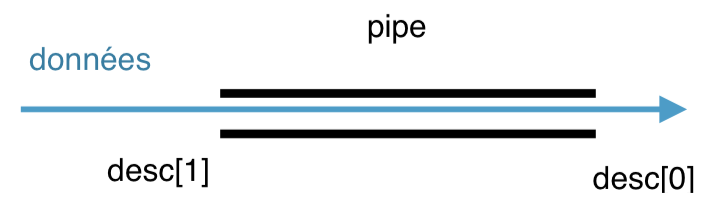
\includegraphics{pipe}

\section{Redirection de tubes aka \emph{dup2( )}}
Vous vous souvenez de \emph{dup2( )}? Vous savez, le cours ou vous avez \sout{rien} tout compris? Eh ben on va en reparler à travers un petit exercice:\footnote{inspiré de http://www.zeitoun.net/articles/communication-par-tuyau/start}\\
\textbf{Bouyou-Geauchamps}: \textit{Faites un programme qui execute l'équivalent de la commande "\emph{ls | wc}", sinon je \textbf{WAWAWAWAWAAAA}}\\

Comme vous êtes des gens vraiment \emph{too stongue}, vous avez certainement les étapes en tête:
\begin{itemize}
\item{Le processus père créé un processus fils, qui exécute \emph{ls}}
\item{La sortie standard du processus fils est \textbf{redirigée} vers l'entrée standard du père}
\item{Le père execute ensuite wc}
\item{\textit{C'est gagné}}
\end{itemize}

L'étape 1 est relativement facile:
\begin{lstlisting}
int main( int argc, char ** argv )
 {
   pid_t pidFils = fork();

   if (pidFils == 0)
     {
       execlp("ls", "ls", NULL);
       return 1;
     }

   wait(NULL);
   execlp("wc", "wc", NULL);
   return 2;
 }
\end{lstlisting}

La difficulté se passe évidemment sur la redirection. Il faut nécessairement créer un pipe qui fera la communication entre le père et le fils - on appellera ce pipe \emph{pipeCom} - mais pour la suite?\\
Comme vous l'avez deviné, il faut utiliser \emph{dup2( )}.\\
\emph{dup2( )} se présente de la manière suivante:
\begin{verbatim}
int dup2(int fdSource, int fdCible);
\end{verbatim}
En fait, \emph{dup2( )} permet de copier le file descriptor en deuxième argument dans le premier.

Dans notre exercice, cela se traduit donc par une \textbf{redirection} de la sortie standard du fils sur l'entrée du pipe \emph{pipeCom} et une redirection de la sortie du pipe \emph{pipeCom} sur l'entrée standard du père.\\ Regardez le schéma pour un peu plus de clarté:\\
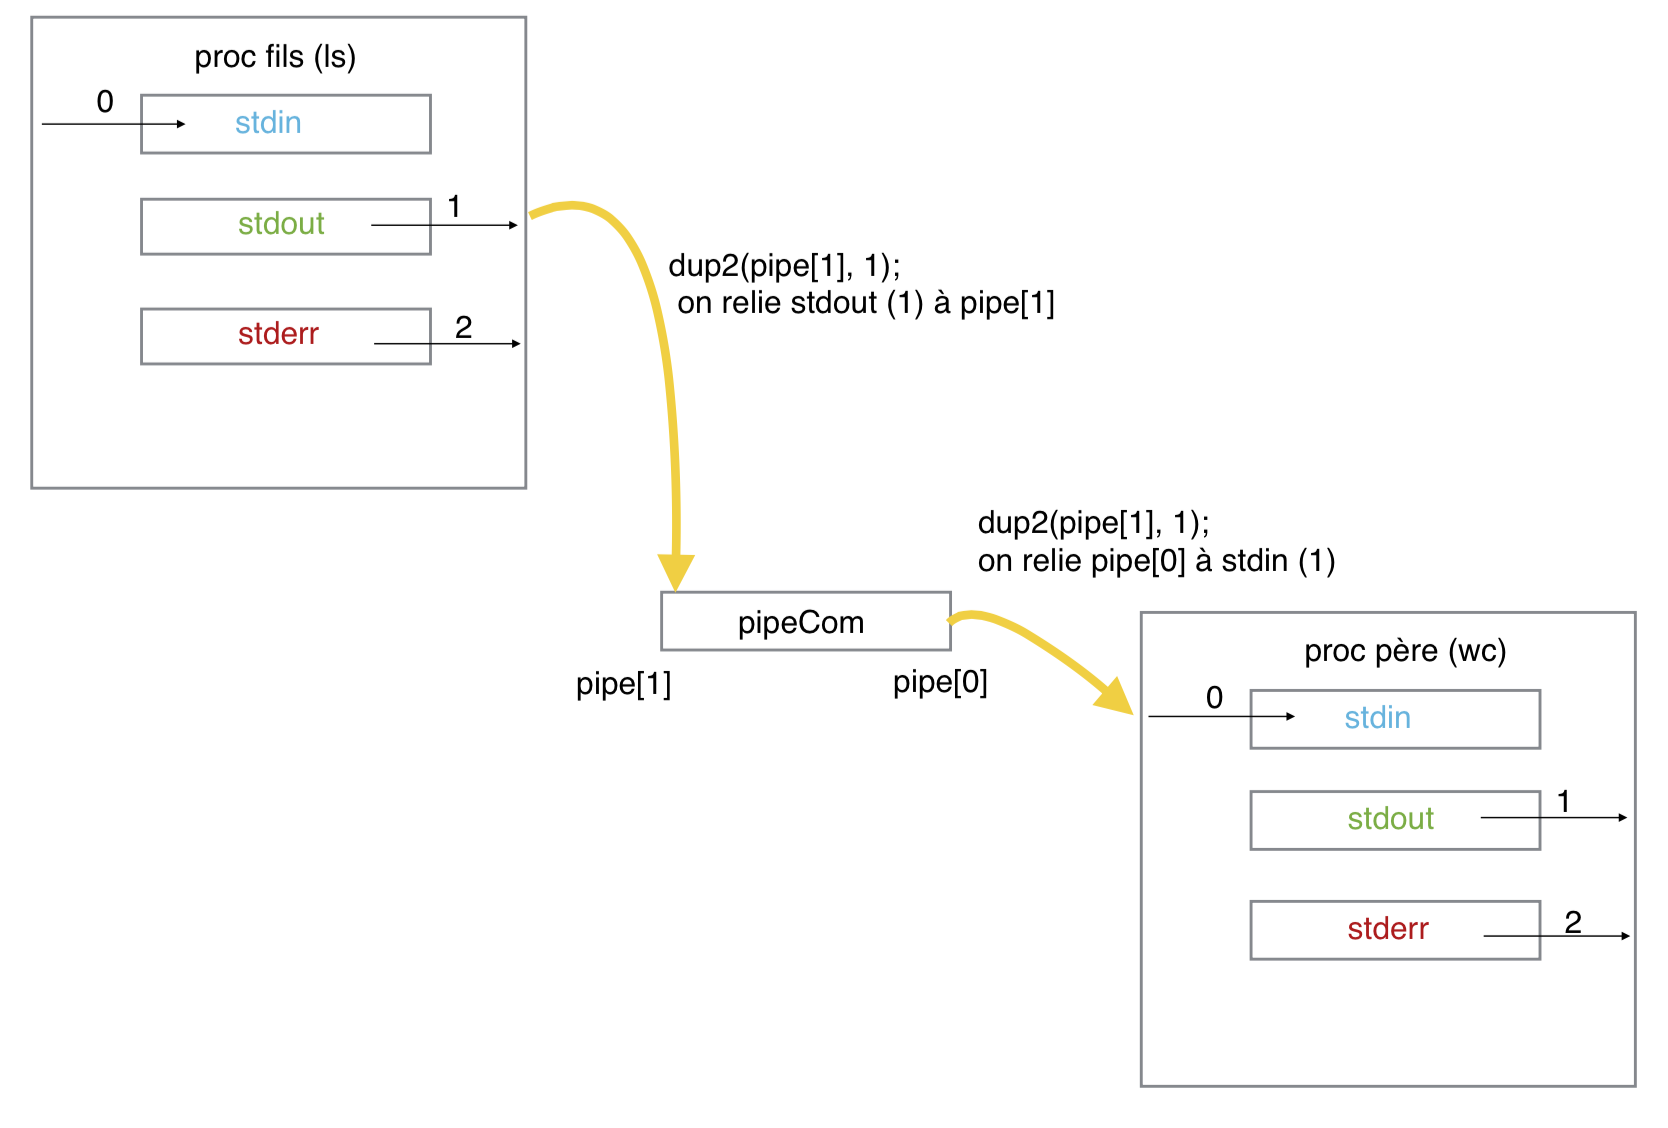
\includegraphics[scale=0.5]{dup2}
\\ Et maintenant, voilà notre code:
\begin{lstlisting}
int main( int argc, char ** argv )
 {
   pid_t pidFils = fork();
   int pipeCom[2];
   pipe(pipeCom);

   if (pidFils == 0)
     {
       close(pipeCom[0]);
       dup2(pipeCom[1],1);
       close(pipeCom[1]);
       execlp("ls", "ls", NULL);
       return 1;
     }

   wait(NULL);
   close(pipeCom[1]);
   dup2(pipeCom[0],0);
   close(pipeCom[0]);
   execlp("wc", "wc", NULL);
   return 2;
 }
\end{lstlisting}
On n'oublie pas de fermer les entrées/sorties inutiles pour éviter des embrouilles, et c'est gagné!



\chapter{Threads (\& Jamy) feat Firegrain ofc}
\epigraph{"JME KASS, ET C TOU"}{McRoss, qui en a visiblement marre des threads}



\section{La notion de thread}
Vous vous souvenez des processus? Un programme englobe des processus, un processus englobe des threads. En fait, un thread est, \emph{une unité d'éxecution plus fine qu'un processus}. Ce n'est pas pour rien qu'on appelle aussi les threads des \emph{processus léger}. La différence majeure avec les processus est que les threads \textbf{partagent tout} entre eux. En effet, lorsque on créé un processus, le fait de modifier quelque chose dans le processus fils n'impactait pas le processus père. Avec les threads, ce n'est pas le cas. Par exemple, si un thread modifie une variable globale, cette variable sera modifiée pour \textbf{tous les threads}. Il faut donc faire attention !

\section{Création de thread}
Pour créer un thread, on utilise la fonction \emph{pthread\_create( )}. Cette fonction se présente de la manière suivante:
\begin{verbatim}
int pthread_create(pthread_t *thread, const pthread_attr_t *attr, void *(*fonc)(void*), void *arg);
\end{verbatim}
Regardons tranquillement les paramètres et leur rôle:
\begin{itemize}
\item{\emph{thread} représente un pointeur (ou une adresse) sur un objet de type \emph{pthread\_t} qui sera l'identifiant du thread après l'execution de cette fonction;}
\item{\emph{attr} représente le ou les attributs du thread, on peut voir ça comme les options de la fonction open(); }
\item{\emph{fonc} représente un \textbf{pointeur de pointeur de fonction} - vous suivez? -. Ça sera la fonction exécutée par le thread.\footnote{Pour simplifier, un pointeur de fonction représente juste une fonction avec une étoile devant le nom. Pas besoin de se compliquer la vie :):):):)};}
\item{\emph{arg} représente un argument passé pour la fonction, il faut que ce soit un pointeur sans type, utiliser un cast si besoin. C'est donc le paramètre que va utiliser le thread pour la fonction donnée précédemment;}
\end{itemize}
Regardons maintenant un exemple:
\begin{lstlisting}
#include<pthread.h>

void *fonction_thread(void *attr)
{
     printf("coucou, tu veux voir mon pthread_t????? \n c'est trop génial");
     
    /* on regarde si le pointeur attribut pointe sur quelque chose */
    if(attr!=NULL) 
    {
    	 /* l'attribut est considéré comme une chaine de caractère */
        printf("l'attribut en string",(char*)attr); 
        /* l'attribut considéré comme un pointeur d'entier */
        printf("l'attribut en int",*((int*)attr)); 
    }
    int retour=0;
    pthread_exit((void*)&retour); 
    /* je quitte et je renvoie l'adresse de ma variable retour en faisant 
     * bien attention de renvoyer un pointeur sans type */
}

int main(int argc, char **argv)
{
	
	printf("Je suis le thread principal et je vais créer un autre thread");
	pthread_t* fredId;
        int param = 5;
	pthread_create(fredId, NULL, fonction_thread, (void*)&param); 
    /* lorsque je passe un pointeur de fonction en paramètre je
     * passe le nom de la fonction, ici je peux faire le malin parce 
     * que la signature de
     * fonction_thread correspond à celle demandé par la signature 
     * de la fonction pthread_create
     * j'envoie aussi l'adresse de param en le considérant comme
     * une adresse sans type */

	printf("Maintenant j'attends la fin du thread");
       int retour;
	pthread_join(fredId, (void *)retour); 
	// et hop je récupère la valeur de retour	
	exit(retour);

}
\end{lstlisting}	

\section{Arrêt forcé d'un Thread}

%Je suis un Thread qui veut arrêter son fils (ou un putain de random qui veux faire chier un autre thread), dans ce cas j'utilse la fonction\newline
Pour arrêter un thread, il faut utiliser:
\begin{verbatim}
int pthread_cancel(pthread_t thread);
\end{verbatim}
avec \emph{thread} étant l'identifiant du thread que vous avez envie d'arrêter. \textbf{Cependant}, tout comme les processus et les signaux, un thread est capable de bloquer cette demande d'arrêt.

\subsection{Modification du comportement lors d'une demande d'arrêt}
Pour modifier ce comportement, il faut utiliser:
\begin{verbatim}
int pthread_setcancelstate(int etat, int *etat_ancien);
\end{verbatim}
Un peu comme \emph{open( )} et ses multiples flags, il est possible de spécifier une ou plusieurs options avec des pipes pour le paramètre etat :
\begin{itemize}
\item{Comportement à la reception du signal : \emph{PTHREAD\_CANCEL\_DISABLE} pour bloquer le signal d'arrêt ou \emph{PTHREAD\_CANCEL\_ENABLE} pour se terminer}
\item{Comportement si je récupère le signal : PTHREAD\_CANCEL\_ASYCHRONOUS pour n'accepter le signal qu'à certains point de contrôle, c'est à dire quand j'utilise la fonction  pthread\_join, pthread\_testcancel ou pthread\_cond\_wait. Et PTHREAD\_CANCEL\_DEFERRED si j'accepte sans attendre le signal. }
\end {itemize}
\begin{dialogue}
\speak{Firegrain} voilà pour l'arret d'un thread
\speak{M.Tourlemonde} attendez vous n'avez pas expliquer le deuxième paremètre
\speak{Firegrain} ah oui, eh bien....
\speak{Toutlemonde} ?
\speak{Firegrain} en fait, on fait on doit spécifier notre comportement précédent, mais vu qu'on ne le connait pas forcement... ce paramètre est un peu useless en somme, en général on met NULL et on s'en porte pas plus mal
\speak{Toutlemonde} dites plutôt que vous ne savez pas ce que c'est
\speak{Firegrain} Oh, ispice di piti!
\speak{...} nous interrompons cette fiche à cause d'un petit problème technique, nous nous reverrons plus tard
\speak{...} Nous dédicassons cette fiche à Firegrain qui a été arrêté suite à atteinte sur mineur... Il est condamné à payer une amende de 12 000 euro, à 3 mois d'emprisonnement et 12 mois de travaux d'intêret général...
\end{dialogue}




\end{document} 